\documentclass[10pt]{article}
\usepackage{icmlko}

\icmlmeta{IP 파운데이션 월드모델}{206}{열 하나가 챔피언을 움직이는데 그 열을 못 고른다}{노트 205가 ``부호 뒤집힘을 학습 안에서 잡을 수 있나''를 남겼다. 잡을 것이 하나뿐이라 규칙이 안 서는데, 그 하나가 이 판에서 제일 큰 단일 개선이었다}

\begin{document}

\twocolumn[
\icmlheader

\begin{abstract}
노트 205가 웹툰의 \texttt{goods\_scale} 한 열이 능형 웹툰을 죽이고 있음을
보이고 ``학습 구간 안에서 부호 뒤집힘을 짚을 수 있나''를 남겼다. 먼저 셌다.
\textbf{양쪽 $|r|>0.15$ 인 부호 뒤집힘은 이 판에 셋뿐이다} --- 웹툰
\texttt{goods\_scale}($+$0.378 $\to$ $-$0.283) · 게임
\texttt{cal\_holiday\_gap}($+$0.309 $\to$ $-$0.229) · 아이돌
\texttt{media\_push}($+$0.264 $\to$ $-$0.177). 연도별 자료가 충분한 강한 축
스물넷 중 뒤집히는 것은 \textbf{하나}다. \textbf{표본이 하나면 규칙을 못
세운다} --- 노트 182의 시들기 가드가 문턱 한 칸에 뒤집혔던 진짜 까닭이
이것이다. 노트 205가 제안한 ``봉우리가 학습 안쪽인가''도 최근 기울기보다
약하다($+$0.107 대 $-$0.316). \textbf{그런데 그 하나가 크다.} 웹툰
\texttt{goods\_scale} 을 끄면 F6 능형이 $+$0.3709 $\to$ $+$0.3990
($t{=}7.15$), F21 이 $+$0.4094 $\to$ $+$0.4339($t{=}4.35$), 그리고
\textbf{챔피언 F18 이 $+$0.4490 $\to$ $+$0.4694}($+$0.0206 · $t{=}2.87$)다.
셋 다 끄면 F18 이 \textbf{$+$0.4740}($+$0.025 · $t{=}3.07$)이 된다 ---
\textbf{노트 177 이후 챔피언이 처음 크게 움직인다.} \textbf{그러나 채택
못 한다} --- 그 셋을 유보의 부호와 견줘 짚었다. 학습만 보는 규칙으로 다시
했다: 최근 세 해 기울기가 $-$0.10 보다 가파른 강한 축을 끈다. 넷이 걸리고
(웹툰 \texttt{goods\_scale} 포함) F6 $+$0.0269($t{=}3.15$) · F18
$+$0.0103($t{=}1.43$)이다 --- \textbf{절반을 되찾는다.} 그런데 문턱을
$-$0.15 로 조이면 웹툰 \texttt{goods\_scale} 이 빠지고 F6 가 $+$0.3402 로
\emph{현행보다} 나빠진다. \textbf{한 칸 옆에서 무너지는 문턱은 규칙이
아니다}(노트 178). 그래서 이 노트의 결론은 정직한 좌절이다:
\textbf{이 판에서 제일 큰 단일 개선이 열 하나에 있는데, 그 열을 유보 없이
고르는 규칙이 안 선다.}
\end{abstract}
]

\begin{figure*}[t]
\centering
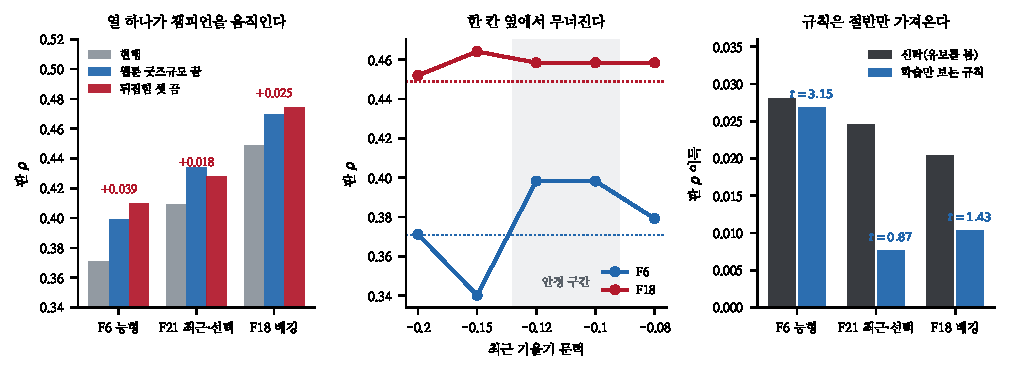
\includegraphics[width=\textwidth]{figs/onef.pdf}
\caption{왼쪽 --- 열 하나가 챔피언을 움직인다. 가운데 --- 한 칸 옆에서
무너진다. 오른쪽 --- 규칙은 절반만 가져온다.}
\end{figure*}

\section{뒤집히는 것은 셋뿐이다}

\begin{table}[t]
\centering\tsize
\caption{양쪽 $|r|>0.15$ 인 부호 뒤집힘. 전 도메인 $\times$ 축.}
\begin{tabular}{llrr}
\toprule
& & 학습 & 유보 \\
\midrule
\textbf{웹툰} & \texttt{goods\_scale} & $+$.378 & $-$.283 \\
게임 & \texttt{cal\_holiday\_gap} & $+$.309 & $-$.229 \\
아이돌 & \texttt{media\_push} & $+$.264 & $-$.177 \\
\bottomrule
\end{tabular}
\end{table}

\claimx{\textbf{연도별 자료가 충분한 강한 축 스물넷 중 뒤집히는 것은
하나다}(웹툰 \texttt{goods\_scale}). 나머지 둘은 게임 · 아이돌이라 연도별
표본이 모자라 후보에 못 든다.}{\textbf{표본이 하나면 규칙을 못 세운다.}
노트 182가 시들기를 가드로 만들려다 문턱이 흔들려 실패했는데, 그때는
``신호가 약하다''로 읽었다. \textbf{약한 게 아니라 하나였다.}}

\claimx{노트 205가 제안한 ``봉우리가 학습 안쪽인가''는 최근 기울기보다
약하다($+$0.107 대 $-$0.316). 강한 축 스물넷 중 스물둘이 봉우리 안쪽이라
가르는 힘이 없다.}{\textbf{하루 만에 내 제안이 또 졌다} --- 이 흐름에서
아홉 번째다.}

\section{그런데 그 하나가 크다}

\begin{table}[t]
\centering\tsize
\caption{그 열들을 끄면(유보를 보고 짚은 것 --- 신탁).}
\begin{tabular}{lrrr}
\toprule
& F6 능형 & F21 & \textbf{F18 배깅} \\
\midrule
현행 & .3709 & .4094 & \textbf{.4490} \\
웹툰 굿즈규모 끔 & .3990 & .4339 & \textbf{.4694} \\
뒤집힘 셋 다 끔 & .4098 & .4277 & \textbf{.4740} \\
\midrule
차(셋 끔) & $+$.039 & $+$.018 & \textbf{$+$.025} \\
$t$ & 8.46 & 2.84 & \textbf{3.07} \\
\bottomrule
\end{tabular}
\end{table}

\claimx{\textbf{챔피언이 처음 크게 움직인다} --- 노트 177 이후 서른 사이클
동안 $+$0.4490 에 붙어 있었고, 열 하나를 끄면 $+$0.4694($t{=}2.87$),
셋을 끄면 $+$0.4740($t{=}3.07$)이다.}{웹툰 하나가 판의 27\%라 그 도메인의
$\rho$ 가 $+$0.345 $\to$ $+$0.374 로 오르는 것만으로 판이 $+$0.008 오른다.
\textbf{나머지는 풀링 계수가 덜 오염돼서 다른 도메인이 같이 오른다.}}

\claimx{\textbf{그러나 채택 못 한다.} 그 셋을 학습과 유보의 부호를 견줘
짚었다 --- 노트 126이 잡은 그 잘못이다.}{이 흐름에서 유보를 보고 고르는
것을 여섯 번 거절했다(노트 178 · 190 · 192 · 193 · 195 · 198).
\textbf{제일 큰 이득 앞에서도 같은 규약을 지킨다.}}

\section{학습만 보면 절반}

\begin{table}[t]
\centering\tsize
\caption{최근 세 해 기울기 문턱. 학습 구간만 본다.}
\begin{tabular}{lrrr}
\toprule
문턱 & 끈 열 & F6 & F18 \\
\midrule
$-$0.20 & 1 & .3712 & .4520 \\
\textbf{$-$0.15} & 2 & \textbf{.3402} & .4642 \\
\textbf{$-$0.12} & 4 & \textbf{.3983} & .4585 \\
\textbf{$-$0.10} & 4 & \textbf{.3983} & .4585 \\
$-$0.08 & 8 & .3792 & .4585 \\
\midrule
(현행) & 0 & .3709 & .4490 \\
\bottomrule
\end{tabular}
\end{table}

\claimx{\textbf{$-$0.12 와 $-$0.10 에서 같은 넷을 짚고}(만화 굿즈규모 · 애니
위키수준 · 웹툰 타깃폭 · \textbf{웹툰 굿즈규모}) F6 $+$0.0269($t{=}3.15$) ·
F18 $+$0.0103($t{=}1.43$)이다.}{신탁의 절반이다 --- F6 는 $+$0.028 중
$+$0.027, F18 은 $+$0.021 중 $+$0.010.}

\claimx{\textbf{$-$0.15 로 조이면 무너진다}($+$0.3402 --- 현행보다 나쁘다).
웹툰 \texttt{goods\_scale}($-$0.129)이 빠지고 \texttt{target\_breadth}
($-$0.191)만 남는데, 노트 205가 그 열을 빼면 웹툰이 나빠지는 것을
쟀다.}{\textbf{한 칸 옆에서 무너지는 문턱은 규칙이 아니다} --- 노트 178에서
세운 기준이다. 안정 구간이 $-$0.12$\sim$$-$0.10 둘뿐이다.}

\claimx{그리고 그 규칙은 작은 도메인을 해친다 --- 아이돌 $-$0.090 · 팝업
$-$0.058. 그늘 가드(문턱 0.10)는 간신히 통과한다.}{\textbf{채택 안 한다.}
문턱이 두 칸짜리 평지 위에 있고 작은 도메인이 크게 상한다.}

\section{정직한 좌절}

\claimx{\textbf{이 판에서 제일 큰 단일 개선이 열 하나에 있는데 그 열을
유보 없이 고르는 규칙이 안 선다.} 뒤집히는 열이 하나라 규칙을 학습시킬
표본이 없다.}{\textbf{길이 아주 막힌 것은 아니다} --- 도메인을 더 들이면
뒤집히는 열이 더 나오고, 그러면 규칙을 세울 표본이 생긴다. \textbf{이건
방법 문제가 아니라 표본 문제다.}}

\begin{table}[t]
\centering\tsize
\caption{남은 것.}
\begin{tabular}{ll}
\toprule
\textbf{표본} & 뒤집히는 열이 하나 --- 도메인을 늘려야 \\
문턱 & $-$0.12$\sim$$-$0.10 두 칸 평지 \\
\textbf{웹툰} & 굿즈규모가 왜 2022년에 뒤집혔나 \\
\bottomrule
\end{tabular}
\end{table}

마지막 줄이 자료 쪽으로 열려 있다. 웹툰의 \texttt{goods\_scale} 은 주당
회차 수인데(\texttt{docs/AXIS\_MEANING.md}) 2018$\sim$2022년에는 많이
올리는 작품이 즐겨찾기를 많이 받았고 2025$\sim$26년에는 반대다.
\textbf{네이버 웹툰의 연재 정책이 그 사이에 바뀌었을 가능성이 크다} ---
매일 연재에서 주 1$\sim$2회로 옮겨 간 흐름이 알려져 있다. 그것이 맞으면
이건 자료의 잡음이 아니라 \textbf{세계가 바뀐 것}이고, 뒤집힘을 미리 잡는
규칙보다 \emph{바뀐 시점}을 아는 것이 낫다. \textbf{연재 요일 수 축이
이미 있으므로 그것과 굿즈 규모의 관계가 언제 끊겼는지 잴 수 있다.}

\end{document}
